\section{Protocolo y corpus}

Los resultados de este capítulo proceden de una única campaña de evaluación sobre el dump NYIT 
\textit{home+lab cleaned} (iPhone XR), sin reentrenamiento posterior a las corridas archivadas en 
\texttt{data/eval\_run/}. El protocolo es \textit{open-set} y \textit{user-disjoint}: 49 usuarios de 
entrenamiento, 16 de desarrollo y 18 de evaluación (\textit{seed} 42). El enrolamiento usa las $k=5$ 
primeras ventanas de cada modalidad; las consultas son el leftover completo. El impostor es aleatorio 
(otros usuarios del mismo split); NYIT no define impostor hábil. La longitud oficial de tecleo es $N=50$. 
El umbral operativo se fija en desarrollo (EER) y se aplica en evaluación. No se persistió texto crudo.

Dos advertencias de lectura son imprescindibles. Primera: el Transformer de tres modalidades se evalúa 
sobre 545 pares genuinos (el tope lo impone el scroll), mientras que el ensemble de tres modalidades y 
las ablaciones de tecleo usan 2278; las curvas y barras no deben compararse como si compartieran el mismo 
$N$. Segunda: TypeNet, Type2Branch y BehaveFormer (Tabla~\ref{tab:baseline}) son SOTA de \textbf{otro} corpus
(Aalto/HuMIdb) y no se dibujan en los mismos ejes que las figuras de este capítulo. El único referente
publicado sobre NYIT es Cariello et al.~\cite{cariello2025posture,cariello2026keystroke}: verificadores
RF/$k$-NN/SVM y, cuando el EER baja del $2\%$, captura Vicon. No existe un Transformer SOTA en este dump
con el que igualar arquitectura y protocolo.

\section{Unimodales}

En evaluación leftover, las modalidades aisladas se sitúan cerca del azar práctico salvo un ligero 
margen del tecleo en el Transformer (EER $44{,}59\%$, AUC $0{,}59$). La firma \textit{proxy} y el scroll 
unimodales rinden EER $47$--$50\%$ (AUC $\approx 0{,}50$). El dump de tecleo es solo \textit{press}: 
el tiempo de pulsación (DT) es nulo y el tiempo de vuelo coincide con el IKI, lo que empobrece la señal 
respecto a TypeNet. La firma no es un trazo legal de rúbrica, sino un \textit{swipe} reutilizado como 
\textit{proxy}.

\section{Ensemble y fusores}

Entre las estrategias de fusión a nivel de \textit{score}, el meta-clasificador es el único que mejora 
de forma clara al experto de tecleo con $z$ reclamado (EER $28{,}98\%$ frente a $30{,}37\%$). Los 
fusores lineal fijo, $1/\mathrm{EER}$ y softmax aprendido quedan por encima del $33\%$ de EER; el 
aprendido ($35{,}69\%$) no supera al fijo. Añadir firma \textit{proxy} y scroll al ensemble con pesos 
fijos \textbf{empeora} el EER respecto a solo tecleo ($36{,}62\%$ frente a $30{,}37\%$). La fusión 
de scores no logra extraer identidad de canales próximos al azar.

\section{Transformer y ablación de scroll}

El Transformer de tres modalidades es el mejor sistema propuesto: EER $24{,}60\%$, AUC $0{,}830$ 
(545 genuinos, 9265 impostores). Al enmascarar el scroll en el mismo \textit{checkpoint} el EER sube a 
$28{,}14\%$ (2278 genuinos): el scroll \textbf{sí} aporta en este enfoque. Enmascarar también la firma 
deja el EER prácticamente igual ($28{,}14\%$), coherente con la nula discriminabilidad unimodal del 
\textit{proxy}. El unimodal de tecleo del Transformer ($44{,}59\%$) es peor que el experto BiLSTM con 
$z$ reclamado en el pipeline fused ($30{,}37\%$), lo que indica que la ganancia del TF está en la 
atención cruzada, no en el encoder de tecleo aislado.

\section{Comparación Transformer frente a ensemble}

Bajo el mismo split de usuarios, el Transformer 3-mod (EER $24{,}60\%$, tasa TTD $97{,}7\%$) supera 
al ensemble meta (EER $28{,}98\%$, tasa TTD $41{,}2\%$). La Figura~\ref{fig:f1_det} muestra el 
compromiso FAR/FRR; la curva IMU (tecleo+IMU) se incluye como réplica, no como candidato propuesto. 
La comparación de EER en la Figura~\ref{fig:f2_eer} resume la misma ordenación, con la salvedad del 
$N$ de pares.

\section{Longitud de secuencia}

La ablación del BiLSTM de tecleo con $N\in\{25,50,100\}$ produce EER $48{,}88\%$, $47{,}56\%$ y 
$46{,}48\%$ (Figura~\ref{fig:f3_seqlen}). Alargar la ventana ayuda poco y no reproduce el salto que 
TypeNet reporta en Aalto a $N=50$. El TTD se mide en número de ventanas, de modo que $N$ mayor retrasa 
la decisión en eventos de tecla aunque el EER baje décimas.

\section{Comparación con Random Forest (mismo protocolo)}

Este experimento no replica Cariello et al.: no hay mocap Vicon, no hay split por sesión del mismo usuario ni ventanas de $1$\,s. Se fija el leftover NYIT de este TFM ($k=5$, $N=50$, impostor aleatorio) y solo cambia el verificador. Un \textit{Random Forest} de rasgos agregados (IKI con DT nulo, vector de scroll $6$-D, descriptores de la serie de firma \textit{proxy}) se ajusta en \textit{dev} y se evalúa en leftover. Un segundo RF (L3) sustituye al meta-clasificador sobre el triplete de \textit{scores} de los expertos congelados. No se ejecutó RF sobre embeddings (L2). Cifras: \texttt{data/rf\_run/index.json}.

En eval leftover el mejor RF es el meta de scores (EER $30{,}32\%$, AUC $0{,}762$). No bate al ensemble meta ($28{,}98\%$) ni al Transformer 3-mod ($24{,}60\%$). El RF de tecleo ($32{,}01\%$) sí mejora el unimodal BiLSTM ($47{,}56\%$). Concatenar firma \textit{proxy} y scroll al RF de rasgos baja poco el EER ($32{,}01\%\to 30{,}95\%$): el canal extra no discrimina, igual que en el ensemble. La Figura~\ref{fig:f7_rf} y la Tabla~\ref{tab:rf_leftover} resumen la ordenación. El $1{,}5\%$ de Cariello \textbf{no} se pinta en el eje. IMU y mocap no entran aquí.

Las probabilidades del bosque L1 no se calibran entre \textit{dev} y \textit{eval}: el $\tau$ de EER de \textit{dev} produce un rechazo casi total en eval. El ranking de sistemas se lee por \textbf{EER eval}, no por ese punto operativo. En L3 el $\tau_{\mathrm{dev}}$ sí da un compromiso (FAR $0{,}34$ / FRR $0{,}21$), aún peor en EER que el meta neuronal.

\begin{table}[H]
\centering
\caption{Random Forest en el leftover propio (eval). No es réplica de Cariello.}\label{tab:rf_leftover}
\begin{tabular}{lccc}
\toprule
\textbf{Sistema} & \textbf{EER (\%)} & \textbf{AUC} & \textbf{Genuinos} \\
\midrule
RF tecleo (L1) & 32{,}01 & 0{,}767 & 2278 \\
RF 3-mod rasgos (L1) & 30{,}95 & 0{,}756 & 2278 \\
RF meta de scores (L3) & 30{,}32 & 0{,}762 & 2278 \\
Ensemble meta 3-mod & 28{,}98 & 0{,}796 & 2278 \\
Transformer 3-mod & 24{,}60 & 0{,}830 & 545 \\
\bottomrule
\end{tabular}
\end{table}

\section{IMU (experimento no propuesto)}

La Tabla~\ref{tab:imu_replica} y la Figura~\ref{fig:f4_imu} recogen la réplica tecleo+IMU. El unimodal 
IMU es azar ($51{,}06\%$); la fusión $1/\mathrm{EER}$ baja el EER de tecleo de $47{,}56\%$ a 
$34{,}63\%$. Esa mejora no entra en la tabla del sistema propuesto. BehaveFormer ($2{,}95\%$ en 
HuMIdb) no es comparable 1:1.

\begin{table}[H]
\centering
\caption{Réplica IMU en NYIT (eval leftover). No es el sistema propuesto.}\label{tab:imu_replica}
\begin{tabular}{lc}
\toprule
\textbf{Sistema} & \textbf{EER (\%)} \\
\midrule
IMU unimodal & 51{,}06 \\
Tecleo unimodal (mismo protocolo) & 47{,}56 \\
Tecleo + IMU ($1/\mathrm{EER}$) & 34{,}63 \\
\bottomrule
\end{tabular}
\end{table}

\section{Discusión frente a Cariello (mismo set) y al SOTA de otro corpus}

Sobre \textbf{este} dump, Cariello et al.\ son el único referente~\cite{cariello2025posture,cariello2026keystroke,NYIT_dataset:2025}.
Sus arquitecturas no son Transformers: plantillas de rasgos y RF, $k$-NN, SVM de una clase o Manhattan
escalada. El EER $\approx 1{,}5\%$ (tecleo, $1$\,s) y el $5{,}4$--$6{,}4\%$ (\textit{swipe}, $1$--$5$\,s)
incluyen mocap de laboratorio (Vicon). El baseline de \textbf{solo teléfono} que ellos mismos publican
queda en $9{,}5$--$11{,}9\%$ (tecleo/IMU, $1$\,s) y $15{,}7\%$ (\textit{swipe}+IMU, $60$\,s). Ni siquiera
ese baseline es 1:1 con este TFM: ellos usan lab, dos sesiones del mismo usuario y ventanas de un segundo
ancladas al evento; aquí el protocolo es \textit{open-set} leftover ($N=50$, press-only, fusión no
simultánea, sin Vicon). Un RF de rasgos y un RF-meta de scores en \textbf{ese} leftover (Tabla~\ref{tab:rf_leftover})
quedan en EER $30$--$32\%$: la cabeza clásica no recupera el $1{,}5\%$ ni supera al Transformer. No hay
un Transformer SOTA en NYIT contra el que medir el $24{,}60\%$ más allá de esta comparación interna.

TypeNet, Type2Branch y BehaveFormer ($\approx 1$--$3\%$ en Aalto/HuMIdb) siguen siendo SOTA \textbf{ajena}:
otro dispositivo, otra señal (DT real, IMU de HuMIdb) y otro protocolo. El ranking interno
(Transformer $>$ ensemble meta $>$ RF-meta $>$ unimodales) es interpretable en NYIT; el salto a operación tipo Aalto
o tipo Vicon no lo es. MobileB2C (AUC mixed $66{,}37\%$ en BehavePassDB) es, de nuevo, otro corpus.

\section{Figuras}

\begin{figure}[H]
\centering
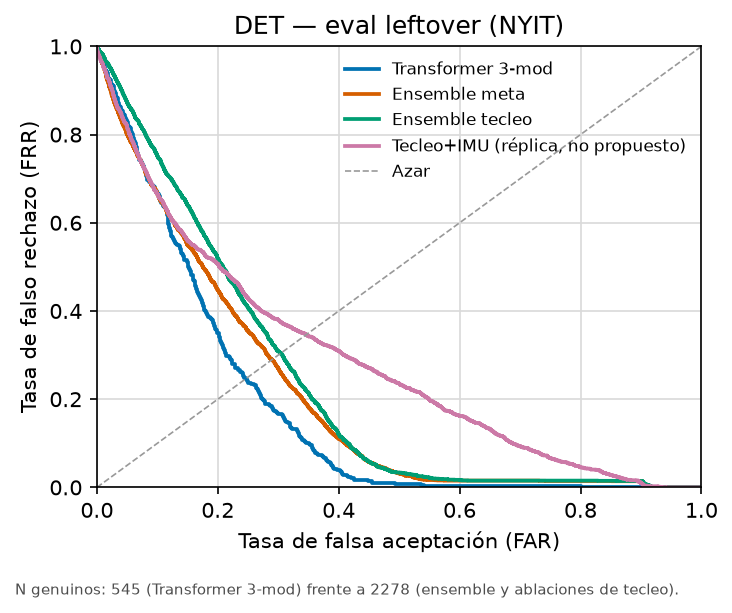
\includegraphics[width=0.92\textwidth]{files/figures/cap06/det_transformer_ensemble.png}
\caption{Curvas DET en evaluación leftover (NYIT). El Transformer 3-mod opera mejor en el compromiso 
FAR/FRR que el ensemble meta. La serie tecleo+IMU es réplica, no propuesta. Nota: 545 frente a 2278 
pares genuinos según sistema.}
\label{fig:f1_det}
\end{figure}

\begin{figure}[H]
\centering
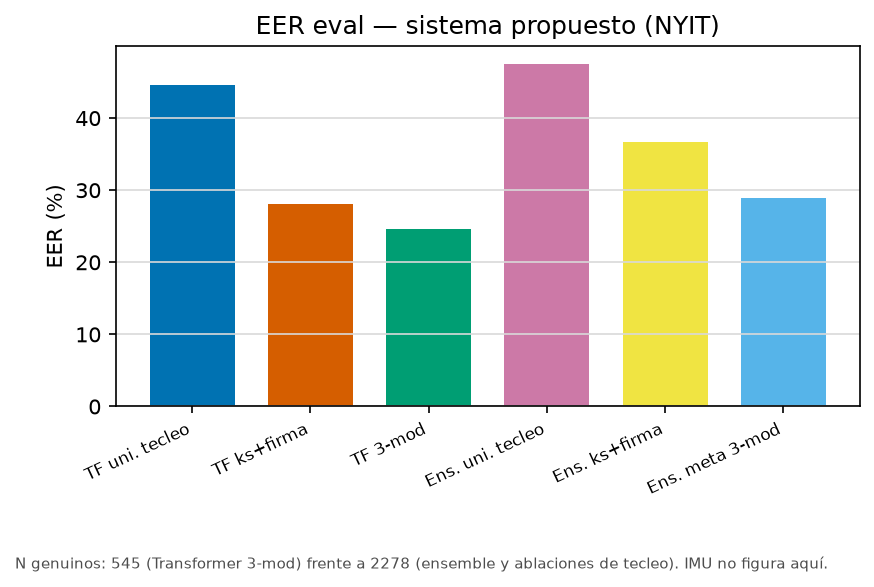
\includegraphics[width=0.92\textwidth]{files/figures/cap06/eer_barras_propuesto.png}
\caption{EER (\%, eval) del sistema propuesto. El scroll reduce el EER del Transformer y no ayuda al 
ensemble. IMU ausente a propósito.}
\label{fig:f2_eer}
\end{figure}

\begin{figure}[H]
\centering
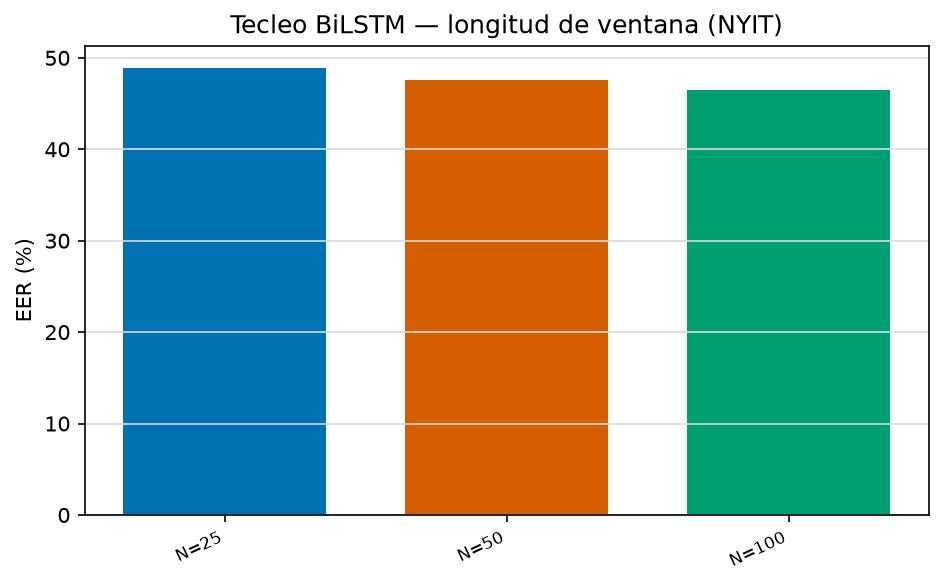
\includegraphics[width=0.85\textwidth]{files/figures/cap06/eer_seqlen.png}
\caption{EER del BiLSTM de tecleo frente a la longitud de ventana. No hay salto comparable al de TypeNet 
en Aalto.}
\label{fig:f3_seqlen}
\end{figure}

\begin{figure}[H]
\centering
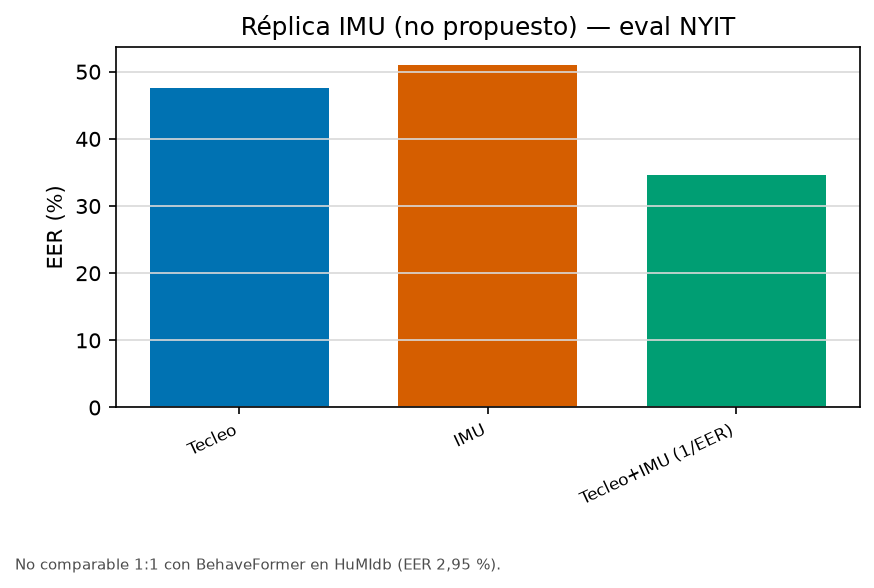
\includegraphics[width=0.85\textwidth]{files/figures/cap06/eer_imu.png}
\caption{EER de la réplica IMU (no propuesto). HuMIdb/BehaveFormer no se pintan en el mismo eje.}
\label{fig:f4_imu}
\end{figure}

\begin{figure}[H]
\centering
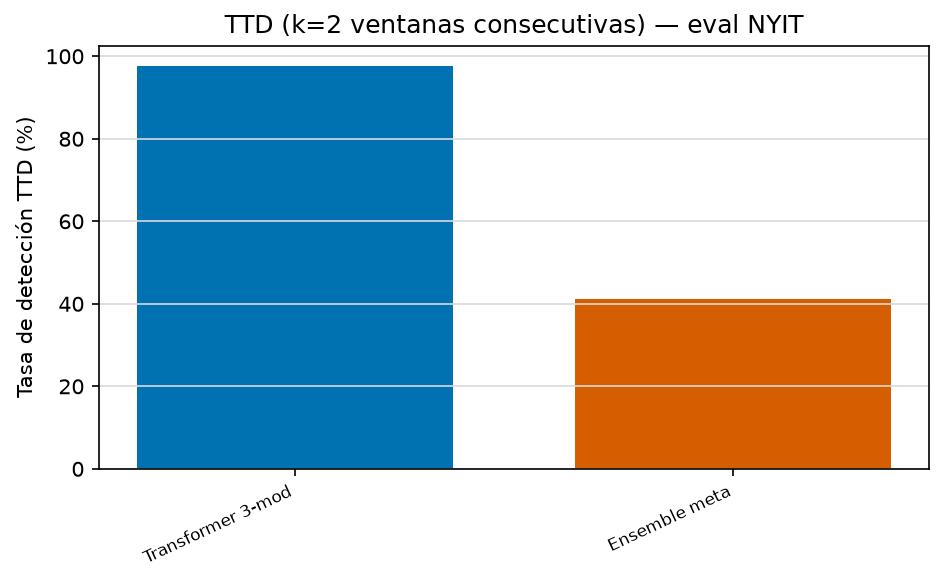
\includegraphics[width=0.75\textwidth]{files/figures/cap06/ttd_detect.png}
\caption{Tasa de detección TTD ($k=2$ ventanas consecutivas). El Transformer marca impostor en más 
secuencias que el ensemble meta.}
\label{fig:f5_ttd}
\end{figure}

\begin{figure}[H]
\centering
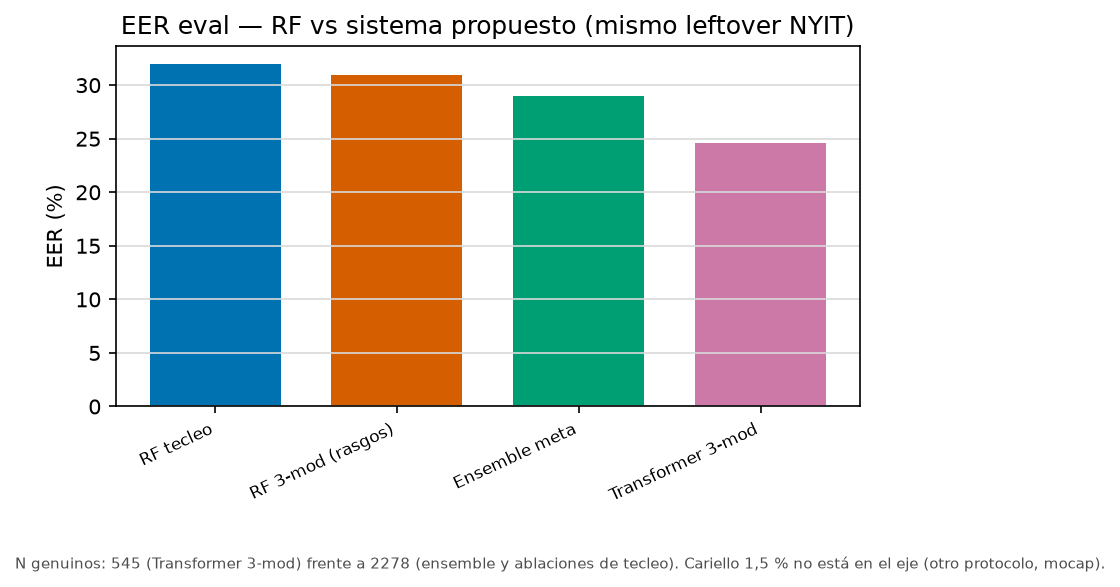
\includegraphics[width=0.92\textwidth]{files/figures/cap06/eer_rf_vs_propuesto.png}
\caption{EER (\%, eval leftover NYIT) del Random Forest de rasgos frente al ensemble meta y al Transformer 3-mod, mismo protocolo. Cariello $1{,}5\%$ no figura en el eje (otro split, mocap). Nota: 545 frente a 2278 pares genuinos según sistema.}
\label{fig:f7_rf}
\end{figure}

\begin{table}[H]
\centering
\caption{Resumen eval leftover del sistema propuesto (EER y AUC). Cifras de \texttt{tables.json}.}\label{tab:eval_propuesto}
\begin{tabular}{lccc}
\toprule
\textbf{Sistema} & \textbf{EER (\%)} & \textbf{AUC} & \textbf{Genuinos} \\
\midrule
Transformer 3-mod & 24{,}60 & 0{,}830 & 545 \\
Transformer tecleo+firma & 28{,}14 & 0{,}796 & 2278 \\
Ensemble meta 3-mod & 28{,}98 & 0{,}796 & 2278 \\
Ensemble solo tecleo ($z$ reclamado) & 30{,}37 & 0{,}773 & 2278 \\
Ensemble tecleo+firma (fijo) & 36{,}62 & 0{,}702 & 2278 \\
Transformer unimodal tecleo & 44{,}59 & 0{,}586 & 2278 \\
\bottomrule
\end{tabular}
\end{table}
